% !TeX root = ../main.tex

\section{Grundlegende Begriffe}

\begin{frame}{Komponenten}
    \alert{\textbf{Identity Provider}} (IdP)
    \vspace{-\topsep}
    \begin{itemize}
        \item Authentifizierung der Benutzer:in über Home-Organisation ~\cite{dfnDFNAAIDokumentationEinfuhrung, shibbolethShibbolethConcepts2023}
        \item bspw. Bildungs- und Forschungseinrichtungen (HTWK)
    \end{itemize}
    
    \pause
    \alert{\textbf{Service Provider}} (SP)
    \vspace{-\topsep}
    \begin{itemize}
        \item Prüfung der Authentifizierung und Autorisierung
        \item Zugriff auf Ressource~\cite{shibbolethServiceProviderApplication2021, shibbolethServiceProviderProtectContent2021, shibbolethShibbolethConcepts2023}
        \item bspw. E-Learning-Plattformen (OPAL), Bibliotheken~\cite{dfnDFNAAIDokumentationEinfuhrung}
    \end{itemize}
    
    \pause
    \alert{\textbf{Discovery Service}} (DS)
    \vspace{-\topsep}
    \begin{itemize}
        \item Unterstützung der SP bei Ermittlung eines geeigneten IdP
        \item \emph{Where Are You From?} (WAYF)~\cite{shibbolethIdPDiscoveryShibbolethConcepts2020, shibbolethShibbolethConcepts2023, switchSimpleDemoSwitchAAI2024}
    \end{itemize}
\end{frame}


\begin{frame}{Grundlegender Prozessablauf}
    \begin{figure}
        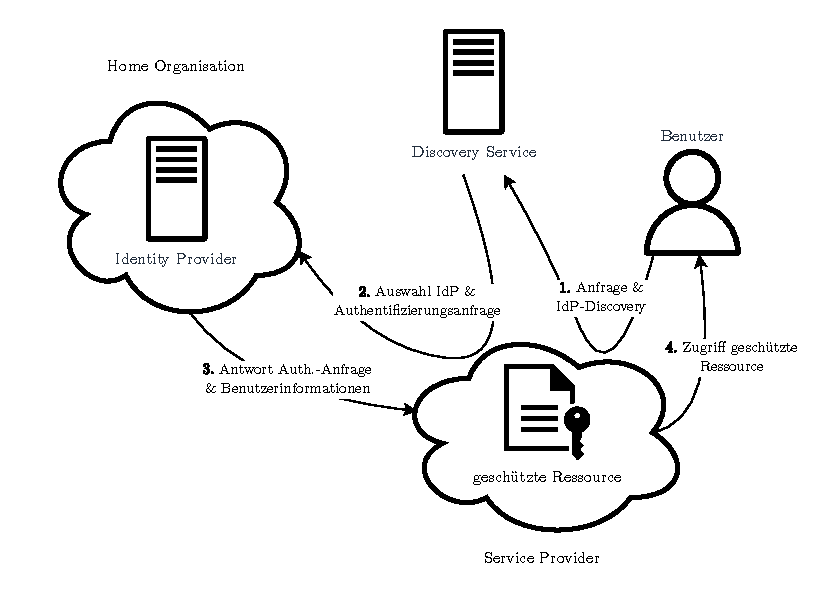
\includegraphics[height=0.7\paperheight]{../assets/basic_interaction_article.drawio.pdf}
        \caption{Grundlegender Prozessablauf~\cite{michelsIdentityManagementUnd, shibbolethShibbolethConcepts2023, switchExpertDemoSWITCHaai2024a}}
    \end{figure}
\end{frame}
